%% ---------------------------------------------------------------------------------------------------------------------

\chapter{Introduction}\label{ch:introduction}

In today's modern society, software has become an integral part of many industries and areas of life.
The security of that software is very important, because successful attacks on it can have serious implications,
especially in the case of critical infrastructures like energy and food supply chains or medical services.
It is therefore important to try reducing the attack surface as best as possible.
Many security problems that exist in software systems are caused by programming errors of some kind.
Programming languages provide various concepts to help avoiding common pitfalls and mistakes that developers make, but
they can not completely prevent them from happening.

This thesis takes a deeper look into the Go programming language and specifically into its \unsafe{} \acrshort{API}.
It analyzes the risk that comes with the use of this language feature, and presents novel software tools that help
developers to identify and minimize it.


%% ---------------------------------------------------------------------------------------------------------------------

\section{Motivation}\label{sec:introduction:motivation}

In the last decade, there has been an ongoing adoption of memory-safe languages for many different applications.
Such languages include for example Google's Go (or Golang), Rust, Nim, or even Java.
Memory safety is one of the most important areas of software security, because a large number of vulnerabilities is
caused by memory access bugs.
In fact, Microsoft for example reports that memory safety accounts for around \checkNum{70\%} of all their
bugs~\footnote{\scriptsize\url{https://msrc-blog.microsoft.com/2019/07/16/a-proactive-approach-to-more-secure-code/}}.
To reduce the risk of such vulnerabilities, many modern languages provide different mechanisms to protect potentially
dangerous operations, such as accessing raw memory, dereferencing raw pointers, or arbitrary conversion between
incompatible types.
However, these languages also provide ways for developers to explicitly circumvent the safety measures to various
degrees.
Go uses a compile-time enforcement of a strict typing system with limiting rules on pointer access and cast operations
and automatic memory management using a garbage collector (\acrshort{GC}) to achieve a high level of memory and thread
safety, but it also offers the \unsafe{} package.
This package is an \acrshort{API} built into the language that allows arbitrary access to raw pointers, similar to the
way pointers in C behave, such as conversions between completely different types and pointer arithmetic.

There are legitimate use cases for this, such as the implementation of a low-level networking protocol that needs
direct access to the raw byte data, or an application with time and memory constraints that needs to cast values to
different types without reallocating them.
Furthermore, \unsafe{} operations might be necessary to access hardware when building e.g. a driver, or to use
foreign function interfaces (\acrshort{FFI}) such as Cgo, providing interoperability between code implemented in
different languages.
It is however dangerous to use the \unsafe{} \acrshort{API} because when used incorrectly it can cause memory safety
bugs that lead to exploitable security vulnerabilities, as is shown in this thesis.
There can be buffer overflows leading to possible code injections when incompatible types with different sizes or
memory alignments are converted into each other, or the compiler may be unable to correctly determine the lifetime of
a value and allocate it on a function stack instead of the program heap, which can can lead to use-after-free
vulnerabilities and thus all kinds of malicious program behaviors.
Thus, when \unsafe{} code is used it must be properly audited by the developers at least.
Furthermore, even after an initial code review it is important that security researchers can effectively analyze the
code base for potential misuses of \unsafe{} code, and administrators who deploy the software to their systems should
be aware of the possible consequences as well.

Checking \unsafe{} code in a project can however be hard because it can be introduced not only through first-party
code, but also through dependencies.
Recently, Evans et al.~\cite{evans2020} showed that in Rust programs \unsafe{} blocks are often introduced through
third-party libraries.
It might not be directly obvious which dependencies contain \unsafe{} code and should be audited, and checking all of
them is tedious and would create a tremendous cost in terms of developer time.
Not knowing about the dangers introduced through the use of external dependencies can however have severe consequences
in terms of security vulnerabilities.
Therefore, security analysts, developers, and administrators need tools that support them in identifying \unsafe{}
code usages in their project including its dependencies and assessing their risk.
There are suitable tools for other languages such as
\toolCargoGeiger{}~\footnote{\url{https://github.com/rust-secure-code/cargo-geiger}} for Rust code, but previously there
was no such tool for Go.
Although there are tools like \toolGosec{}~\footnote{\url{https://github.com/securego/gosec}} that provide limited
ability to identify \unsafe{} usages in a single package, they can not analyze the dependencies of the package.

This thesis presents the design and implementation as well as an evaluation of two novel developer tools for this
purpose.
\toolGeiger{} can find and count \unsafe{} usages in a Go package and its dependencies and is therefore similar in its
design to \toolCargoGeiger{}.
The linter tool \toolSafer{} identifies \unsafe{} usage patterns that are dangerous and common in real-world Go code.
Its design is based on a security analysis of code samples that use the \unsafe{} \acrshort{API}, which was conducted as
part of this thesis as well.
Using \toolGeiger{}, we also present a study of the current state of \unsafe{} usage in popular open-source Go projects.
This allows researchers and developers to understand how many usages there are in the first place, how they are
introduced, what is being done in \unsafe{} call sites, and for what purpose.
Based on that knowledge, informed decisions can be made on whether or not to use specific third-party libraries, or how
a code review process for a particular organization should be designed to achieve the best performance.
To draw a big picture, the goal of this thesis is to analyze and improve the reality of \unsafe{} code in software
projects written in the Go programming language.



%% ---------------------------------------------------------------------------------------------------------------------

\section{Contributions}\label{sec:introduction:contributions}

This section lists and briefly outlines the main contributions that are made in this thesis.
They are the following:

\begin{enumerate}
    \item A thorough analysis of problems and consequences of usage patterns of the \unsafe{} \acrshort{API} in Go code
    with respect to a security context, revealing \checkNum{three} main areas of danger,

    \item \toolGeiger, a novel open-source static analysis tool to identify and count \unsafe{} usages in Go packages
    including their dependencies,

    \item a quantitative study of \unsafe{} code usage in \projsAnalyzed{} of the top \projsTotal{} most popular
    open-source Go projects on \github{},

    \item an in-depth study of \numberLabeledCodeSnippets{} code samples used in \projsForLabeledCodeSnippets{} selected
    projects, yielding a two-dimensional manual classification of usages and valuable insight into how and for what
    purpose unsafe code is used in Go applications,

    \item \toolSafer{}, a novel open-source, \toolVet{}-style, linter tool to find \checkNum{two} dangerous and common
    \unsafe{} usage patterns that were previously uncaught with existing tools, including an evaluation of its
    performance,

    \item the submission of \numberPRs{} pull requests to project maintainers with fixes to more than
    \numberBugsFixedRounded{} previously vulnerable code snippets in open-source Go libraries, \numberPRsMerged{} of
    which have been merged by the authors so far, and

    \item a replication of a related study on \unsafe{} Go code in concurrent work by Costa et al.~\cite{costa2020},
    including a comparison to this work and discussion of differences.
\end{enumerate}


%% ---------------------------------------------------------------------------------------------------------------------

\section{Outline}\label{sec:introduction:outline}

The remainder of this thesis is structured as described in the following: Chapter~\ref{ch:background} gives background
information on memory safety and the Go \unsafe{} \acrshort{API}, as well as the dependency management system used in
Go and static code analysis.
Chapter~\ref{ch:unsafe-security-problems} analyzes and discusses possible vulnerabilities caused by \unsafe{} code
usages which can be found in real-world application code, including the development of proof-of-concept exploit code.
Then, Chapter~\ref{ch:go-geiger} presents the design, implementation, and evaluation of \toolGeiger, a novel static
analysis tool which finds and counts \unsafe{} usages in a Go package as well as its dependencies.
The chapter also describes the methodology and results for the empirical study analyzing the top \projsTotal{} most
popular open-source Go projects on \github{}, and presents the labeled data set of \numberLabeledCodeSnippets{} code
samples, which categorizes \unsafe{} usages by what is being done and for what purpose.
After that, Chapter~\ref{ch:go-safer} shows the design, implementation, and evaluation of \toolSafer, the novel linter
tool that can identify \checkNum{two} dangerous and common \unsafe{} usage patterns.
Next, Chapter~\ref{ch:related-work} discusses related and concurrent work, including amongst others the replication of
and comparison to a similar study on \unsafe{} usage in Go by Costa et al.~\cite{costa2020}.
Chapter~\ref{ch:discussion} puts the findings and results of this work in context and discusses their meaning and
impact.
Threats to validity and possible future work are also presented there.
Finally, Chapter~\ref{ch:conclusion} concludes the work.

Figure~\ref{fig:outline} shows a visual outline and the relationship between the individual chapters of this thesis.
The relevant chapters contain a version of this figure with the respective parts highlighted to assist in following
along.

\begin{figure}[htp!]
    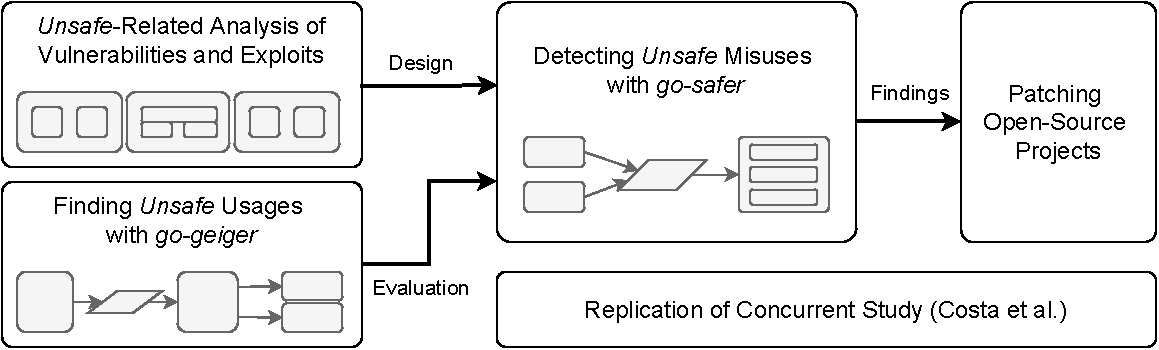
\includegraphics[width=\textwidth]{assets/figures/chapter1/outline1.pdf}
    \caption[Problem statement and thesis organization]
    {Problem statement and thesis organization.\newline\footnotesize~Parts in gray outline chapters and are shown in detail there.}
    \label{fig:outline1}
\end{figure}


It is worth noting that this thesis does not use the typical structure of presenting a design, an implementation, and
lastly an evaluation.
Instead, both software tools \toolGeiger{} and \toolSafer{} have their own design, implementation, and evaluation
sections in their respective chapters.
The necessary theoretical work based on the background information discussed in Chapter~\ref{ch:background} is presented
in its own chapter before introducing the tools.
Furthermore, the methodology and results of the study on \unsafe{} code in open-source Go projects is presented in
Chapter~\ref{ch:go-geiger} alongside the \toolGeiger{} tool, because first, the study data is gathered using \toolGeiger,
and second, it simultaneously serves as an evaluation of \toolGeiger{}.
